\section{Details of Approach}
Within the approach we followed the implementations of GLOW. We followed the
implementation detailed within the GLOW paper. The basic architecture is shown
in Figure~\ref{fig:glowarch}.

\begin{figure}
    \begin{subfigure}[]{\columnwidth}
        \center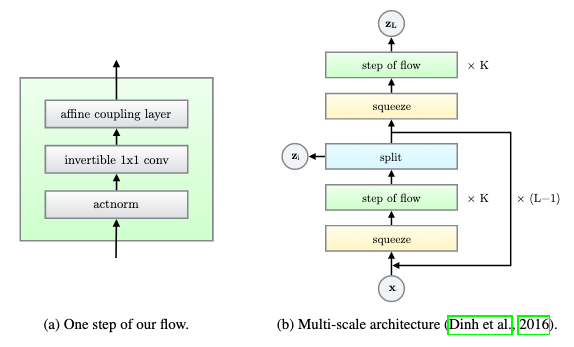
\includegraphics[width=\columnwidth]{GLOWFlow.png}
    \end{subfigure}
    %
    \begin{subfigure}[]{\columnwidth}
        % offsets by 2 because GLOWFlow has (a) and (b) already
        \addtocounter{subfigure}{2} 
        \center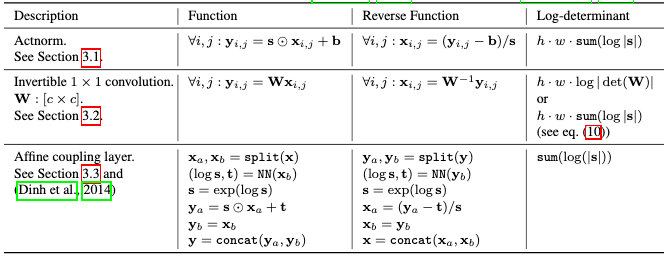
\includegraphics[width=\columnwidth]{GLOWComposition.png}
        \caption{Components of network architecture}
        \label{fig:glowcomp}
    \end{subfigure}
    \caption{GLOW Architecture}
    \label{fig:glowarch}
\end{figure}

From this diagram we can see that for the most part the inner workings of GLOW
are fairly simple. To implement it each of these was abstracted out into a
different class so that they could be chained together. Each bold variable, that
doesn't have a subscript, in Figure~\ref{fig:glowcomp} represents a learned
parameter. 
\subsection{Actnorm}
%
In the Actnorm layer of Figure~\ref{fig:glowcomp} we see
that there's the equation
%
\begin{equation}
 \forall i,j : \mathbf{y}_{i,j} = \mathbf{s} \odot \mathbf{x}_{i,j} + \mathbf{b}
\end{equation}
%
we see that $\mathbf{y}$ and $\mathbf{x}$ are tensor components but $\mathbf{s}$
and $\mathbf{b}$ are learned parameters that use the form
\lstinline[basicstyle=\ttfamily]|torch.nn.Parameter()|. Here
\lstinline[basicstyle=\ttfamily]|Parameter()| is initialized with either 
\lstinline[basicstyle=\ttfamily]|torch.ones(1, channels, 1, 1)|, $\mathbf{s}$, or
\lstinline[basicstyle=\ttfamily]|torch.zeros(1, channels, 1, 1)|, $\mathbf{b}$.
$\mathbf{s}$ is defined with ones and $\mathbf{b}$ is defined with zeros so that
each parameter initially starts as a no-op, no scaling nor transformation.
The reverse function is similarly defined, using the same parameters, by using
the \lstinline[basicstyle=\ttfamily]|backward| function. The Log-determinant is
defined withing the \lstinline[basicstyle=\ttfamily]|forward| and
\lstinline[basicstyle=\ttfamily]|backward| functions.

\subsection{Invertible $1\times 1$ Convolutional Layer}
%
The GLOW paper defines the Invertible $1\times 1$ Convolutional
Layer as a rotation matrix, which is why it substitutes for a permutation
between flow layers. To accomplish this we used torch's 
\lstinline[basicstyle=\ttfamily]|nn.init.orthogonal_()| function to generate a
randomized $2\times 2$ matrix that would be orthogonal. By initializing it as
orthogonal we help set it up to be a rotation matrix, which are frequently
orthonormal. Meaning that they only perform a permutation operation on another
matrix and do not scale or transform. We then use this in torch's
\lstinline[basicstyle=\ttfamily]|conv2d()| function from the Functional library.
This allows for a convolutional layer to be generated but we're able to
initialize the weight matrix. This makes building the permutation layer pretty
easy. 

\subsection{Affine Coupling Layer}
%
The major challenge we had in building the flow steps was tackling the
Affine Coupling Layer. While it looks simple, there are many aspects to it that
are not well defined in the GLOW paper nor the RealNVP paper, which is
frequently referenced. The initial operation, $\mathbf{x}_a, \mathbf{x}_b =
split(\mathbf{x})$, is similar to NICE. The second operation,
$(\log{\mathbf{s}}, \mathbf{t}) = NN(\mathbf{x}_b)$, is composed of a coupling
layer that has several actnorm and convolutional layers, finishing with a
scaling layer. This is almost exactly like the flow layers described in NICE. At
the end of this layer we return two values, which are split along the channel.
From there we finish with another actnorm layer and concat with the original
split, such that one half is processed through the actnorm and another through
the $NN()$.

\subsection{Multi-Scale Architecture}
Once we have our flow steps define the structure for the multi-scale
architecture needed to be created. The \lstinline[basicstyle=\ttfamily]|squeeze|
layer is defined by reshape, permutation, and a reshape. Here we looked at the
source code and found that the operation is performed by reshaping the input as
\lstinline[basicstyle=\ttfamily]|(-1, C, H//2, 2, W//2, 2)| -- where C = the channels, H =
height and W = width --, a permutation of \lstinline[basicstyle=\ttfamily]|(0,1,3,5,4)| --
meaning that we have a tensor of shape 
\lstinline[basicstyle=\ttfamily]|(batch, channel, 2, 2, H//2, W//2)| 
-- and finally another reshape,
\lstinline[basicstyle=\ttfamily]|(-1, 4*C, H//2, W//2)|. This performs a checkerboard
operation, shown in Figure~\ref{fig:checkerboard}, that squeezes the height and
width of the input tensor into the channel dimension.
%
\begin{figure}
\center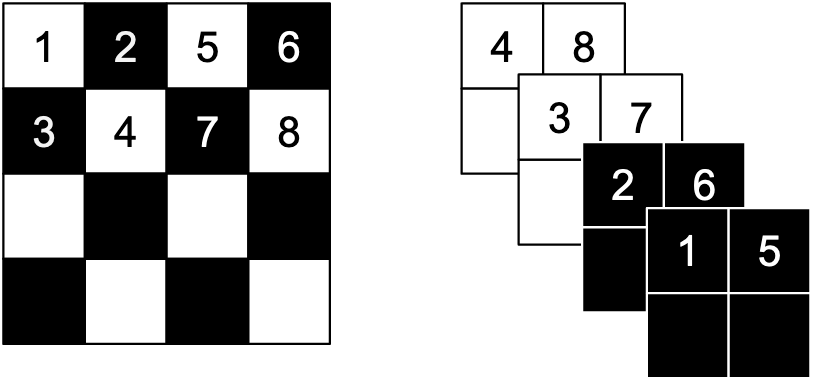
\includegraphics[width=\columnwidth]{checkerboard.png}
\caption{Checkerboard Squeeze operation defined in RealNVP}
\label{fig:checkerboard}
\end{figure}
%
Finally, for each layer we need to perform the split operation. Here we split
each input $\mathbf{x}$ channel-wise into two variables. We then take the mean
of the first and get the log-standard-deviation. The second parameter we use the
following equation:
%
\begin{equation}
    \mathbf{z} = (\mathbf{x_2} - \mu)e^{-log(\sigma)}
\end{equation}
%
Where $x_2$ is one of the splits. The log-determinant is defined as the sum of
the negative log-standard-deviation. 

\subsection{Training}
%
Now that we have all the components of the Normalizing Flow architecture
defined, we can train our network. This is simply done as we connect the
architecture as defined in Figure~\ref{fig:glowarch} and then perform our change
of variables operation. Because of computational restraints we did not build a
network that was as deep as GLOWs. Instead we used 24 steps of flow and 4
layers. We used an Adam optimized with a learning rate of $10^{-4}$. We use a
normal distribution to for our network to learn from. To train the network we
use a similar pattern to more conventional architectures. The difference here is
that we sample from our normal distribution and then send that sample through
our flow network. The difference is that our backwards function,
\lstinline[basicstyle=\ttfamily]|loss.backward()|, goes through the network
backwards and performs the gradient descent. Because normalizing flows are
unsupervised networks, we do not need to calculate a mean square error or some
other criterion at the end. To get our generated results we simply sample from
the normal distribution and send it through the backwards function of the
network. 
